% SECTION: Grundlagen der Statistik
\section{Grundlagen der Statistik}

\divider

% SUBSECTION: Grundbegriffe der Wahrscheinlichkeitstheorie
\subsection{Grundbegriffe der Wahrscheinlichkeitstheorie}

% Wahrscheinlichkeitsräume
\begin{frame}{Wahrscheinlichkeitsräume}{}
	Wir definieren zunächst, was man unter einem \keyword{Wahrscheinlichkeitsraum} versteht.
	\begin{itemize}
		\item Ein Wahrscheinlichkeitsraum ist ein Tripel $(\Omega, \sA, \Prob)$.
		\item $\Omega$ ist der \keyword{Ereignisraum}, also die Menge aller Elementarereignisse.
			Beim Werfen eines sechsseitigen Würfels betrachten wir $\Omega \coloneqq \{ 1, 2, 3, 4, 5, 6 \}$.
		\item Mit $\sA$ bezeichnen wir die zugehörige \keyword{Sigma-Algebra}, eine Menge von Teilmengen von $\Omega$.
			Im einfachsten Fall könnten wir $\sA \coloneqq \Pot(\Omega)$ wählen, jedoch kann man zeigen,
			dass die Potenzmenge im Allgemeinen nicht messbare Mengen enthält,
			denen keine Wahrscheinlichkeit zugeordnet werden kann. Die Sigma-Algebra $\B$ auf $\R$ heißt \keyword{Borel-Sigma-Algebra}.
		\item $\Prob : \sA \rightarrow [0, 1]$ ist ein \keyword{Wahrscheinlichkeitsmaß},
			das jedem Element aus $\sA$ eine Wahrscheinlichkeit zuordnet.
	\end{itemize}
\end{frame}


% Zufallsvariablen
\begin{frame}{Zufallsvariablen}{}
	Im Folgenden sei $(\Omega, \sA, \Prob)$ ein Wahrscheinlichkeitsraum und $(\sX, \sB)$ ein messbarer Raum.
	
	\begin{mydef}[def:random-variable]
		Die Abbildung $X : \Omega \rightarrow \sX$ heißt \keyword{Zufallsvariable}, falls
		\begin{equation*}
			\forall B \in \sB : X^{-1}(B) \coloneqq \{ \omega \in \Omega : X(\omega) \in B \} \in \sA
		\end{equation*}
		gilt. Das Urbild von $B$ unter $X$ muss also eine messbare Menge in $\sA$ sein,
		der durch $\Prob$ eine Wahrscheinlichkeit zugeordnet werden kann.
		Ferner heißt für jede Zufallsvariable $X : \Omega \rightarrow \sX$ die Funktion
		\begin{equation*}
			\Prob^X : \sB \rightarrow [0, 1] \qquad\text{mit}\qquad B \mapsto \Prob\bigl( X^{-1}(B) \bigr)
		\end{equation*}
		die \keyword{Verteilung} der Zufallsvariable $X$. $\Prob^X$ ist das \keyword{Bildmaß} von $\Prob$ unter $X$.
	\end{mydef}
\end{frame}


% Zufallsvariablen (Forts.)
\begin{frame}{Zufallsvariablen (Forts.)}{}
	Sei $(\sX, \sB, \Q)$ ein Wahrscheinlichkeitsraum. Man sagt, die Zufallsgröße $X : \Omega \rightarrow \sX$ ist
	\textit{verteilt gemäß $\Q$} oder kurz \textit{$\Q$-verteilt}, falls es einen Wahrscheinlichkeitsraum $(\Omega, \sA, \Prob)$ gibt,
	sodass $\Prob^X = \Q$ gilt.
	
	\begin{boxGray}
		\textbf{Beispiel:}
		$X$ ist $\norm(\mu, \sigma^2)$-verteilt genau dann, wenn es einen Wahrscheinlichkeitsraum $(\Omega, \sA, \Prob)$ gibt,
		sodass $\forall B \in \B : \Prob(X \in B) = \norm(B; \mu, \sigma^2)$. Wir schreiben kurz $X \sim \norm(\mu, \sigma^2)$.
	\end{boxGray}
\end{frame}


% Wahrscheinlichkeitsdichten
\begin{frame}{Wahrscheinlichkeitsdichten}{}
	\begin{mydef}[def:density]
		Es seien $(\Omega, \sA, \Prob)$ und $(\sX, \sB, \Prob^X)$ Wahrscheinlichkeitsräume.
		Dabei ist $\Prob^X$ die Verteilung der Zufallsvariablen $X : \Omega \rightarrow \sX$.
		Wir nennen eine nichtnegative Funktion $$p_X : \R \rightarrow [0, \infty)$$ eine \keyword{(Wahrscheinlichkeits-)Dichte} von $\Prob^X$, falls
		\begin{equation*}
			\Prob^X(B) = \int_B p_X(\xi)\,\diff\xi \qquad \forall B \in \sB.
		\end{equation*}
	\end{mydef}

	\begin{boxGray}
		\textbf{Bemerkung:} Die Wahrscheinlichkeiten der Mengen $B \in \sB$ müssen sich also allesamt als Integral
		der Dichte $p_X$ darstellen lassen können.
	\end{boxGray}
\end{frame}


% Erwartungswert von Zufallsvariablen
\begin{frame}{Erwartungswert von Zufallsvariablen}{}
	\begin{mydef}[def:expectation]
		Sei $X \in \R$ eine Zufallsvariable. Wir definieren den \keyword{Erwartungswert} (erstes Moment) von $X$ als
		\begin{equation*}
			\E[X] \coloneqq \int_{\R} \xi \cdot p_X(\xi)\,\diff\xi.
		\end{equation*}
	\end{mydef}

	Aus der Linearität des Integrals folgt die des Erwartungswerts, d.\,h. für zwei Zufallsvariablen $X$ und $Y$ und eine beliebige aber feste Zahl
	$\alpha \in \R$ (keine Zufallsvariable!) gelten
	\begin{equation*}
		\E[X + Y] = \E[X] + \E[Y] \qquad\text{und}\qquad \E[\alpha \cdot X] = \alpha \cdot \E[X].
	\end{equation*}
	Wir definieren den Erwartungswert einer vektorwertigen Zufallsvariablen $\bx = (x_1, x_2, \ldots, x_n)^\top$ als
	\begin{equation*}
		\E[\bx] \coloneqq \bigl( \E[x_1], \E[x_2], \ldots, \E[x_n] \bigr)^\top.
	\end{equation*}
\end{frame}


% Varianz von Zufallsvariablen
\begin{frame}{Varianz von Zufallsvariablen}{}
	\begin{mydef}[def:variance]
		Die Varianz einer Zufallsvariablen $X \in \R$ ist definiert als die \textit{erwartete quadratische Abweichung vom Erwartungswert}
		(zweites zentriertes Moment), also
		\begin{equation*}
			\V[X] \coloneqq \E\bigl[ (X - \E[X])^2 \bigr] = \int_\R \bigl( \xi - \E[X] \bigr)^2 \cdot p_X(\xi)\,\diff\xi.
		\end{equation*}
	\end{mydef}

	Unter Ausnutzung der Linearität des Erwartungswerts können wir die Varianz folgendermaßen umschreiben:
	\begin{align*}
		\V[X]
			&= \E\bigl[ (X - \E[X])^2 \bigr] = \E\bigl[ X^2 - 2X \cdot \E[X] + \E[X]^2 \bigr]
	\\[2mm]
			&= \E\bigl[ X^2 \bigr] - 2 \cdot \E[X]^2 + \E[X]^2
				= \E\bigl[ X^2 \bigr] - \E[X]^2.
	\end{align*}
\end{frame}


% Varianz von Zufallsvariablen (Forts.)
\begin{frame}{Varianz von Zufallsvariablen (Forts.)}{}
	Ein paar Bemerkungen. Seien dazu $X$ und $Y$ reelle Zufallsvariablen und $\alpha \in \R$ beliebig aber fest.
	
	\begin{boxGray}
		Die Varianz ist \textbf{nicht} linear!
		\begin{itemize}
			\item Es gilt $\V[X + Y] = \V[X] + \V[Y]$ nur, wenn $X$ und $Y$ unkorreliert sind (\keyword{Satz von Bienaymé}).
			\item $\V[\alpha \cdot X] = \alpha^2 \cdot \V[X]$.
		\end{itemize}
	\end{boxGray}

	\begin{boxGray}
		Eine Verschiebung verändert die Varianz nicht, also $\V[X + \alpha] = \V[X]$ ($\alpha$ ist hierbei keine Zufallsvariable, sondern eine
		konstante reelle Zahl).
	\end{boxGray}
\end{frame}


% Kovarianz
\begin{frame}{Kovarianz}{}
	\begin{mydef}[def:covariance]
		Es seien $X$ und $Y$ zwei Zufallsvariablen. Die \keyword{Kovarianz} zwischen $X$ und $Y$ ist definiert als
		\begin{equation*}
			\Cov[X, Y] \coloneqq \E\bigl[ (X - \E[X]) (Y - \E[Y]) \bigr].
		\end{equation*}
	\end{mydef}

	\begin{boxGray}
		\textbf{Bemerkungen:}
		\begin{itemize}
			\item Die Erwartungswerte müssen natürlich existieren, damit Definition \ref{def:covariance} Sinn ergibt.
			\item Die Kovarianz ist symmetrisch: Es ist \Cov[X, Y] = \Cov[Y, X].
		\end{itemize}
	\end{boxGray}
	
	\begin{mytask}
		Was ist der Unterschied zwischen Kovarianz und Korrelation?
	\end{mytask}
\end{frame}


% Streuungsmatrix
\begin{frame}{Streuungsmatrix}{}
	\begin{mydef}[def:dispersion-matrix]
		Es sei $\bx \in \R^n$ ein Zufallsvektor. Wir definieren die \keyword{Streuungsmatrix} $\D[\bx]$ als
		\begin{equation*}
			\D[\bx] \coloneqq \E\bigl[ (\bx - \E[\bx]) (\bx - \E[\bx])^\top \bigr] \in \R^{n \times n}.
		\end{equation*}
	\end{mydef}

	Für die Einträge von $\D[\bx]$ gilt:
	\begin{align*}
		\bigl( \D[\bx] \bigr)_{ij}
			&= \E\bigl[ (x_i - \E[x_i]) (x_j - \E[x_j]) \bigr]
	\\[2mm]
			&= \E\bigl[ (x_j - \E[x_j]) (x_i - \E[x_i]) \bigr]
			= \bigl( \D[\bx] \bigr)_{ji} =
			\begin{cases}
				\Cov[x_i, x_j] & \text{für}\ i \ne j \\
				\V[x_i] & \text{für}\ i = j.
			\end{cases}
	\end{align*}

	\begin{mytask}
		Zeigen Sie, dass $\D[\bx]$ positiv semidefinit ist.
	\end{mytask}
\end{frame}


% Kovarianzmatrix
\begin{frame}{Kovarianzmatrix}{}
	\begin{mydef}[def:covariance-matrix]
		Es seien $\bx \in \R^n$ und $\by \in \R^m$ zwei Zufallsvektoren. Die \keyword{Kovarianzmatrix} von $\bx$ und $\by$ ist
		\begin{equation*}
			\Cov[\bx, \by] \coloneqq \E\bigl[ (\bx - \E[\bx]) (\by - \E[\by])^\top \bigr] \in \R^{n \times m}.
		\end{equation*} 
	\end{mydef}
\end{frame}


% Diskrete Verteilungen
\begin{frame}{Diskrete Verteilungen}{}
	Einige bekannte diskrete Verteilungen lauten:
	\begin{table}
	\renewcommand{\arraystretch}{1.6}
	\centering
	\begin{tabular}{l | c | l | c | c}
		Name der Verteilung			&	$\Prob^x$		& 	Zähldichte $p_x(k)$										& $\E[x]$ 				&	$\V[x]$
	\\ \hline
		Binomialverteilung			&	$B_{n, p}$ 	& 	${n \choose k} \cdot p^k \cdot (1 - p)^{n - k}$ 					& $n \cdot p$ 			&	$n \cdot p \cdot (1 - p)$
	\\
		Hypergeometrische Verteilung	&	$H_{n, K, N}$	& 	$\frac{{K \choose k} \cdot {N - K \choose n - k}}{{N \choose n}}$ 		& $n \cdot \frac{K}{N}$	&	$n \cdot \frac{K}{N} \cdot (1 - \frac{K}{N}) \cdot \frac{N - n}{N - 1}$
	\\
		Poisson-Verteilung			&	$P_\lambda$ 	& 	$e^{-\lambda} \cdot \frac{\lambda^k}{k!}$						& $\lambda$ 			& 	$\lambda$
	\end{tabular}
\end{table}
\end{frame}


% Absolutstetige Verteilungen
\begin{frame}{Absolutstetige Verteilungen}{}
	\begin{table}
	\renewcommand{\arraystretch}{1.6}
	\centering
	\begin{tabular}{l | c | l | c | c}
		Name der Verteilung			&	$\Prob^x$				& 	Lebesgue-Dichte $p_x(\xi)$																								& $\E[x]$ 				&	$\V[x]$
	\\ \hline
		Normalverteilung			&	$N_{\mu, \sigma^2}$		& 	$\frac{1}{\sqrt{2 \pi \sigma^2}} \cdot e^{-\frac{(\xi - \mu)^2}{2 \sigma^2}}$														& $\mu$ 				& 	$\sigma^2$
	\\
		Gammaverteilung 			& 	$\Gamma_{\lambda, r}$ 	&	$\frac{\lambda^r}{\Gamma(r)} \cdot \xi^{r - 1} \cdot e^{-\frac{\xi}{2}} \cdot \indicator_{[0, \infty)}(\xi)$									& $\frac{r}{\lambda}$ 	& 	$\frac{r}{\lambda^2}$
	\\
		Chiquadrat-Verteilung			& 	$\chi_f^2$ 			& 	$\frac{1}{2^{\frac{f}{2}} \cdot \Gamma\left( \frac{f}{2} \right)} \cdot \xi^{\frac{f}{2} - 1} \cdot e^{-\frac{\xi}{2}} \cdot \indicator_{[0, \infty)}(\xi)$	& $f$					& 	$2 \cdot f$
	\\
		Exponentialverteilung			&	$Exp_\lambda$ 			&	$\lambda \cdot e^{-\lambda \xi} \cdot \indicator_{[0, \infty)}(\xi)$ 																& $\frac{1}{\lambda}$	& 	$\frac{1}{\lambda^2}$
	\\
		Betaverteilung 				& 	$\beta_{a, b}$ 			& 	$\frac{\Gamma(a + b)}{\Gamma(a) \cdot \Gamma(b)} \cdot \xi^{a - 1} \cdot (1 - \xi)^{b - 1} \cdot \indicator_{(0, 1)}(\xi)$ 						& $\frac{a}{a + b}$ 		&	$\frac{a \cdot b}{(a + b)^2 \cdot (a + b + 1)}$
	\\
		Gleichverteilung 				& 	$U_{(a, b)}$			& 	$\frac{1}{b - a} \cdot \indicator_{(a, b)}(\xi)$ 																				& $\frac{a + b}{2}$ 		& 	$\frac{(b - a)^2}{12}$ 
	\end{tabular}
\end{table}
\end{frame}


% Stochastische Unabhängigkeit
\begin{frame}{Stochastische Unabhängigkeit}{}
	Mit Dichten können wir auch die \keyword{stochastische Unabhängigkeit} von Zufallsvariablen definieren:
	
	\begin{mydef}[def:independence]
		Es seien $X \in \R$ und $Y \in \R$ reelle Zufallsvariablen mit den Verteilungen $\Prob^X, \Prob^Y$ und den Dichten $p_X$ bzw. $p_Y$.

		$X$ und $Y$ heißen \keyword{stochastisch unabhängig} genau dann wenn $p_{X, Y} \coloneqq p_X \cdot p_Y$
		eine \keyword{Produktdichte} der Verteilung $\Prob^{X, Y}$ ist, d.\,h. die gemeinsame Dichte von $X$ und $Y$
		ergibt sich als Produkt der Einzeldichten. 
	\end{mydef}

	\begin{boxGray}
		\textbf{Bemerkung:} Stochastisch unabhängige Zufallsvariablen sind auch unkorreliert. \textbf{Die Umkehrung gilt im Allgemeinen nicht!}
		Somit ist die stochastische Unabhängigkeit eine stärkere Forderung als die der Unkorreliertheit.
	\end{boxGray}
\end{frame}


% Bedingte Wahrscheinlichkeiten
\begin{frame}{Bedingte Wahrscheinlichkeiten}{}
	\begin{itemize}
		\item Wahrscheinlichkeiten von Ereignissen verändern sich, wenn wir zusätzliches Wissen mit einbeziehen.
		\item Wir definieren daher:
	\end{itemize}
	\begin{mydef}[def:cond-prop]
		Es seien $X$ und $Y$ zwei Zufallsvariablen, wobei wir den Wert von $Y$ bereits beobachtet haben (Vorwissen).
		Dann ist die \keyword{Wahrscheinlichkeitsdichte von $X$ gegeben $Y$}, in Notation $p(X \mid Y)$, definiert als
		\begin{equation*}
			p(X \mid Y) \coloneqq \frac{p(X, Y)}{p(Y)}.
		\end{equation*}
	\end{mydef}
\end{frame}


% Satz von Bayes
\begin{frame}{Satz von Bayes}{}
	Mit bedingten Wahrscheinlichkeiten können wir einen zentralen Satz der Wahrscheinlichkeitsrechnung angeben:
	\begin{mytheo}[th:bayes]
		Es seien $X$ und $Y$ zwei Zufallsvariablen. Es gilt der \keyword{Satz von Bayes}
		\begin{equation*}
			p(X \mid Y) = \frac{p(Y \mid X) \cdot p(X)}{p(Y)}.
		\end{equation*}
	\end{mytheo}

	\begin{myproof}
		Mit Definition \ref{def:cond-prop} gilt $p(X \mid Y) = \frac{p(X, Y)}{p(Y)}$. Analog gilt $p(Y \mid X) = \frac{p(Y, X)}{p(X)}$.
		Da $p(X, Y) = p(Y, X)$, können wir beide Gleichungen nach der Verbunddichte $p(X, Y)$ auflösen. Wir erhalten also
		$p(X, Y) = p(X \mid Y) \cdot p(Y)$ und $p(X, Y) = p(Y \mid X) \cdot p(X)$. Gleichsetzen liefert schließlich
		\begin{equation*}
			p(X \mid Y) \cdot p(Y) = p(Y \mid X) \cdot p(X)
		\qquad\Longleftrightarrow\qquad
			p(X \mid Y) = \frac{p(Y \mid X) \cdot p(X)}{p(Y)},
		\end{equation*}
		die Behauptung.
	\end{myproof}
\end{frame}


% SUBSECTION: Transformationssatz
\subsection{Transformationssatz}

% Transformationssatz für Lebsgue-Dichten
\begin{frame}{Transformationssatz für Lebesgue-Dichten}{}
	\begin{mytheo}[th:transformation]
		Es seien $\bx$ und $\by$ $n$-dimensionale Zufallsvektoren mit dem Zusammenhang
		\begin{equation*}
			\by = \bT(\bx).
		\end{equation*}
		Die Abbildung $\bT : \R^n \rightarrow \R^n$ sei \textit{bijektiv}, sodass die Umkehrabbildung $\bx = \bT^{-1}(\by)$
		existiert und eindeutig ist. Dann gilt für die Dichte $p_{\by}$ der transformierten Zufallsvariablen $\by$
		\begin{equation*}
			p_{\by}(\by) = p_{\bx}\bigl( \bT^{-1}(\by) \bigr) \cdot \bigl\vert \det J\bT^{-1}(\by) \bigr\vert,
		\end{equation*}
		wobei $p_{\bx}$ die Dichte von $\bx$ und $J \bT^{-1}$ die Jacobi-Matrix der Abbildung $\bT^{-1}$ bezeichnet.
	\end{mytheo}
	
	\begin{myproof}
		Für den Beweis werden Argumente aus der Maß- und Integrationstheorie benötigt, deren Behandlung den Rahmen dieses Kurses übersteigt.
	\end{myproof}
\end{frame}


% Beispiel I
\begin{frame}{Beispiel I}{}
	Es sei $X \sim Exp_2$ eine exponentialverteilte Zufallsvariable mit Ankunftsrate $\lambda = 2$. \\
	Gesucht ist die Dichte der Zufallsvariablen $Y \coloneqq 5X + 2$.
	
	\begin{boxGray}
		\textbf{Lösung:}
		
		Es ist $T(X) \coloneqq 5X + 2$ eine bijektive Transformation mit der Umkehrabbildung
		$X = T^{-1}(Y) = \frac{1}{5}(Y - 2)$.
		Zusammen mit der Dichte $p_X(x) = 2 \cdot e^{-2 x} \cdot \indicator_{[0, \infty)}(x)$ der $Exp_2$-Verteilung
		erhalten wir für die Dichte $p_Y(y)$ der transformierten Zufallsvariablen $Y$
		\begin{align*}
			p_Y(y)
				&= p_X\bigl( T^{-1}(y) \bigr) \cdot \bigl( T^{-1} \bigr)'(y)
					= 2 \cdot e^{-2 \left( \frac{y}{5} - \frac{2}{5} \right)}
						\cdot \indicator_{[0, \infty)}\left(\frac{1}{5} y - \frac{2}{5} \right) \cdot \frac{1}{5}
		\\[2mm]
				&= \frac{2}{5} \cdot e^{\frac{4}{5}} \cdot e^{-\frac{2 y}{5}} \cdot \indicator_{[2, \infty)}(y).
		\end{align*}
	\end{boxGray}
\end{frame}


% Beispiel II
\begin{frame}{Beispiel II}{}
	Der Zufallsvektor $\bx \in \R^n$ habe eine beliebige Lebesgue-Dichte $p_{\bx}$. Die Transformation $\bT$ sei linear und bijektiv,
	also von der Form $\by = \bT(\bx) = \bA \bx + \bb$. Wie lautet die Dichte von $\by$?
	
	\begin{boxGray}
		\textbf{Lösung:}
		
		Unter obigen Voraussetzungen ist $\bA$ invertierbar. Also existiert die Umkehrfunktion, welche durch
		$\bx = \bT^{-1}(\by) = \bA^{-1} (\by - \bb)$ gegeben ist. Als Jacobi-Matrix erhält man $J\bT^{-1}(\by) = \bA^{-1}$.
		
		Die Anwendung der Transformationsformel \ref{th:transformation} ergibt daher für die Dichte $p_{\by}$ von $\by$ den Ausdruck
		\begin{equation*}
			p_{\by}(\by) = \frac{1}{\vert \det \bA \vert} \cdot p_{\bx}\bigl( \bA^{-1} (\by - \bb) \bigr),
		\end{equation*}
		wobei wir den Zusammenhang $\det\bigl( \bA^{-1} \bigr) = \frac{1}{\det \bA}$ benutzt haben.
	\end{boxGray}
\end{frame}


% Beispiel III
\begin{frame}{Beispiel III}{}
	Das nächste Beispiel wird als Übungsaufgabe gestellt:
	\begin{mytask}
		Es sei $X$ eine Zufallsvariable, die $\chi_2^2$-verteilt ist.

		\begin{enumerate}
			\item Berechnen Sie die Lebesgue-Dichte der Zufallsvariable $Y \coloneqq \sqrt{X}$.
			\item Berechnen Sie die Wahrscheinlichkeit $\Prob(Y > \frac{1}{2})$.
		\end{enumerate}
	\end{mytask}
\end{frame}


% SUBSECTION: Multivariate Normalverteilung
\subsection{Multivariate Normalverteilung}

% Multivariate Normalverteilung
\begin{frame}{Multivariate Normalverteilung}{}
	Die multivariate Normalverteilung spielt im weiteren Verlauf eine zentrale Rolle:
	\begin{mytheo}[th:std-norm-mv]
		Es sei $\bx \coloneqq (x_1, x_2, \ldots, x_n)^\top \in \R^n$ ein Zufallsvektor, dessen Komponenten $x_i \in \R$ unabhängig und
		identisch standardnormalverteilt sind, d.\,h. $x_i \sim \norm(0, 1)\,\forall i \in \{ 1, \ldots, n \}$.
		
		Die Dichte der \keyword{multivariaten Standardnormalverteilung} ist dann gegeben durch
		\begin{equation*}
			p_{\bx}(\bx) \coloneqq \frac{1}{(2 \pi)^{\frac{n}{2}}} \cdot \exp\left( -\frac{\Vert \bx \Vert^2}{2} \right).
		\end{equation*}
	\end{mytheo}

	\begin{myproof}
		Wegen der Unabhängigkeit der Komponenten gilt für die Verbunddichte
		\begin{equation*}
			p_{\bx}(\bx)
				= \prod_{i=1}^n p_{x_i}(x_i)
				= \prod_{i=1}^n \frac{1}{\sqrt{2 \pi}} \cdot \exp\left( -\frac{x_i^2}{2} \right)
				= \frac{1}{(2 \pi)^{\frac{n}{2}}} \cdot \exp\left( -\frac{\sum_{i=1}^n x_i^2}{2} \right)
				= \frac{1}{(2 \pi)^{\frac{n}{2}}} \cdot \exp\left( -\frac{\bx^\top \bx}{2} \right)
				= \frac{1}{(2 \pi)^{\frac{n}{2}}} \cdot \exp\left( -\frac{\Vert \bx \Vert^2}{2} \right).
		\end{equation*}
	\end{myproof}
\end{frame}


% Multivariate Normalverteilung (Forts.)
\begin{frame}{Multivariate Normalverteilung (Forts.)}{}
	Für die multivariate Standardnormalverteilung gilt $\E[\bx] = \0$ und $\D[\bx] = \bI$.

	Wir verallgemeinern dies auf beliebige Erwartungswertvektoren $\bmu \in \R^n$ und Streuungsmatrizen $\bSigma \in \R^{n \times n}$.
	Wir fordern lediglich, dass die Streuungsmatrix $\bSigma$ \textit{positiv definit} ist, dass also
	$\bz^\top \bSigma \bz > 0\, \forall \bz \in \R^n \backslash \{ \0 \}$ gilt.

	\begin{enumerate}
		\item Aufgrund der positiven Definitheit von $\bSigma$ gibt es eine untere Dreiecksmatrix $\bA$ mit $\bSigma = \bA \bA^\top$
			(Stichwort: \keyword{Cholesky-Zerlegung}).
		\item Wir betrachten die Transformation $\by \coloneqq \bA \bx + \bmu$. Es gilt
		\begin{equation*}
			\E[\by]
				= \E[\bA \bx + \bmu] = \bA \E[\bx] + \bmu = \bmu \qquad\text{und}
		\qquad
			\D[\by]
				= \D[\bA \bx + \bmu] = \bA \D[\bx] \bA^\top = \bA \bA^\top = \bSigma.
		\end{equation*}
		\item Nun wenden wir die Transformationsformel \ref{th:transformation} an, um die Dichte von $\by$ zu bestimmen.
	\end{enumerate}
\end{frame}


% Multivariate Normalverteilung (Forts.)
\begin{frame}{Multivariate Normalverteilung (Forts.)}{}
	\textbf{Zu Schritt 3:} Es ist $\bT^{-1}(\bx) = \bA^{-1} (\by - \bmu)$. Mit Beispiel II zum Transformationssatz erhalten wir
	\begin{equation*}
		\bigl\vert \det J \bT^{-1}(\by) \bigr\vert = \bigl\vert \det \bA^{-1} \bigr\vert = \frac{1}{\vert \det \bA \vert}.
	\end{equation*}
	Außerdem gilt mit dem Determinantenmultiplikationssatz die Identität
	$\det \bSigma = \det\bigl( \bA \bA^\top \bigr) = \det \bA \cdot \det \bA = \det^2 \bA$.
	Durch Ziehen der Wurzel auf beiden Seiten erhalten wir also $\vert \det \bA \vert = (\det \bSigma)^{\frac{1}{2}}$. 
	Die Dichte $p_{\by}$ nimmt damit die Form
	\begin{equation*}
		p_{\by}(\by) = \frac{1}{(\det \bSigma)^\frac{1}{2}} \cdot p_{\bx}\bigl( \bA^{-1} (\by - \bmu) \bigr)
	\end{equation*}
	an, wobei $p_{\bx}$ die Dichte der Standardnormalverteilung aus Satz \ref{th:std-norm-mv} ist. Wir setzen dort
	$\bx \coloneqq \bA^{-1} (\by - \bmu)$, sodass
	$\Vert \bx \Vert^2 = (\by - \bmu)^\top \bigl(\bA^{-1})^\top \bA^{-1} (\by - \bmu) = (\by - \bmu)^\top \bSigma^{-1} (\by - \bmu)$ gilt. 
\end{frame}


% Multivariate Normalverteilung (Forts.)
\begin{frame}{Multivariate Normalverteilung (Forts.)}{}
	Wir fassen zusammen:
	
	\begin{mydef}[def:norm-mv]
		Es sei $\bmu \in \R^n$ ein Vektor und $\bSigma \in \R^{n \times n}$ eine \textit{positiv definite} Matrix.
		
		Die Dichte der \keyword{multivariaten Normalverteilung} $\norm(\bmu, \bSigma)$ ist gegeben durch
		\begin{equation*}
			p_{\bx}(\bx) \coloneqq \frac{1}{(2 \pi)^{\frac{n}{2}} \cdot (\det \bSigma)^{\frac{1}{2}}} \cdot \exp\left(
				-\frac{1}{2} (\bx - \bmu)^\top \bSigma^{-1} (\bx - \bmu)
			\right).
		\end{equation*}
	\end{mydef}
	
	\begin{boxGray}
		\textbf{Bemerkung:} Die positive Definitheit der Matrix $\bSigma$ impliziert auch deren Invertierbarkeit
		(siehe hierzu Satz \ref{th:col-rank-inv}).
	\end{boxGray}
\end{frame}


% Visualisierung: Multivariate Normalverteilung
\begin{frame}{Visualisierung: Multivariate Normalverteilung}{}
	tbd
\end{frame}


% Partitionierte Normalverteilung
\begin{frame}{Partitionierte Normalverteilung}{}
	\begin{mydef}[def:partitioned-norm]
		Es seien $\bx \in \R^d$ und $\by \in \R^{(n - d)}$ zwei Zufallsvektoren.
		Wir fassen diese zu einem neuen Zufallsvektor $\bz \coloneqq \bigl( \bx^\top, \by^\top \bigr)^\top \in \R^n$
		mit $\bz \sim \norm(\bmu, \bSigma)$ zusammen. Hierbei seien
		\begin{equation*}
			\bmu
				\coloneqq \begin{pmatrix} \bmu_{\bx} \\ \bmu_{\by} \end{pmatrix}
		\qquad\text{und}\qquad
			\bSigma
				\coloneqq \begin{pmatrix} \bSigma_{\bx\bx} & \bSigma_{\bx\by} \\ \bSigma_{\by\bx} & \bSigma_{\by\by} \end{pmatrix}.
		\end{equation*}
		Wir nennen dieses Modell \keyword{partitionierte Normalverteilung}.
	\end{mydef}
	
	\begin{boxGray}
		\textbf{Bemerkungen:} Aus der Symmetrie von $\bSigma$ folgt die von $\bSigma_{\bx\bx}$ und $\bSigma_{\by\by}$.
		Außerdem gilt $\bSigma_{\bx\by} = \bSigma_{\by\bx}^\top$.
		
		Oft ist es einfacher mit der Inversen der Kovarianzmatrix zu arbeiten. Wir definieren daher $\bLambda \coloneqq \bSigma^{-1}$.
		Man nennt diese Matrix \keyword{Präzisionsmatrix}.
	\end{boxGray}
\end{frame}


% Bedingte Normalverteilung
\begin{frame}{Bedingte Normalverteilung}{}
	\begin{mytheo}[th:cond-norm]
		Wir betrachten das Modell der partitionierten Normalverteilung aus Definition \ref{def:partitioned-norm}.
		Für die Zufallsvariable $\bx \mid \by$ gilt
		\begin{equation*}
			\bx \mid \by \sim \norm(\bmu_{\bx\,\mid\,\by}, \bSigma_{\bx\,\mid\,\by}),
		\end{equation*}
		wobei für die Parameter der folgende Zusammenhang gilt:
		\begin{align*}
			\bmu_{\bx\,\mid\,\by}
				&\coloneqq \bmu_{\bx} + \bSigma_{\bx\by} \bSigma_{\by\by}^{-1}(\by - \mu_{\by})
		\\[2mm]
			\bSigma_{\bx\,\mid\,\by}
				&\coloneqq \bSigma_{\bx\bx} - \bSigma_{\bx\by} \bSigma_{\by\by}^{-1} \bSigma_{\by\bx}.
		\end{align*}
		Die Dichte dieser Verteilung bezeichnen wir mit $p_{\bx\,\mid\,\by}$.
	\end{mytheo}

	\begin{myproof}
		Einen Beweis dieser Aussage finden Sie in \cite{Bishop2006} auf den Seiten 85--87.
	\end{myproof}
\end{frame}


% Visualisierung: Bedingte Normalverteilung
\begin{frame}{Visualisierung: Bedingte Normalverteilung}{}
	\begin{figure}[H]
		\divideTwo{0.49}{
			\centering
			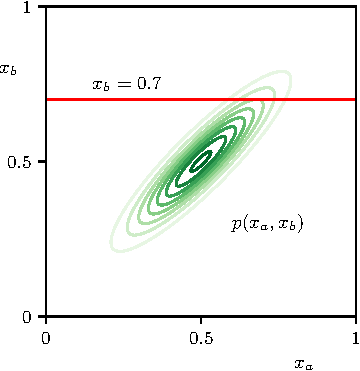
\includegraphics[scale=0.8]{./img/statistics/mv_gaussian.pdf}
		}{0.49}{
			\centering
			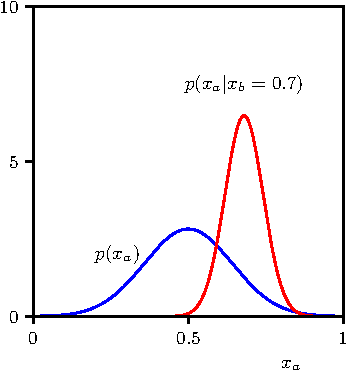
\includegraphics[scale=0.8]{./img/statistics/mv_gaussian_operations.pdf}
		}
		\caption{Links: Zweidimensionale Normalverteilung. Rechts: Bedingte Verteilung in rot. Siehe \cite{Bishop2024}, Seite 82.}
	\end{figure}
\end{frame}


% Aufgabe: Bedingte Normalverteilung
\begin{frame}{Aufgabe: Bedingte Normalverteilung}{}
	\begin{mytask}[task:cond-norm]
		Es sei $\bmu \coloneqq \bigl( 0, 2 \bigr)^\top \in \R^2$ und
		\begin{equation*}
			\bSigma \coloneqq \begin{pmatrix} 0.3 & -1 \\ -1 & 5 \end{pmatrix} \in \R^{2 \times 2},
		\end{equation*}
		sodass die Verbunddichte von $X_1$ und $X_2$ gegeben ist durch $p(X_1, X_2) \coloneqq \norm(\bmu, \bSigma)$.
		Bestimmen Sie die Dichte der bedingten Verteilung $p(X_1 \mid X_2 = -1)$. Benutzen Sie hierzu die Formeln aus Satz \ref{th:cond-norm}.
	\end{mytask}
\end{frame}


% Normale Randverteilung
\begin{frame}{Normale Randverteilung}
	\begin{mytheo}[th:rand-nv]
		Erneut betrachten wir das Modell der partitionierten Normalverteilung aus Definition \ref{def:partitioned-norm}.
		Dann sind auch die Randverteilungen von $\bx$ und $\by$ normalverteilt. Es gilt genauer
		\begin{align*}
			\bx
				&\sim \norm(\bmu_{\bx}, \bSigma_{\bx\bx})
		\\[2mm]
			\by
				&\sim \norm(\bmu_{\by}, \bSigma_{\by\by})
		\end{align*}
		Die Dichten der Randverteilung bezeichnen wir mit $p_{\bx}$ und $p_{\by}$.
	\end{mytheo}

	\begin{myproof}
		Man erhält dieses Ergebnis durch \keyword{Marginalisierung} der Verbunddichte, d.\,h. wir integrieren über alle Variablen,
		die uns nicht interessieren. Für die Randverteilung von $\bx$ gilt zum Beispiel
		\begin{equation*}
			p_{\bx}(\bx) = \int p_{\bx, \by}(\bx, \by)\,\diff \by.
		\end{equation*}
		Einen ausführlichen Beweis finden Sie in \cite{Bishop2006} auf den Seiten 88--89.
	\end{myproof}
\end{frame}


% Visualisierung: Normale Randverteilung
\begin{frame}{Visualisierung: Normale Randverteilung}{}
	\begin{figure}[H]
		\divideTwo{0.49}{
			\centering
			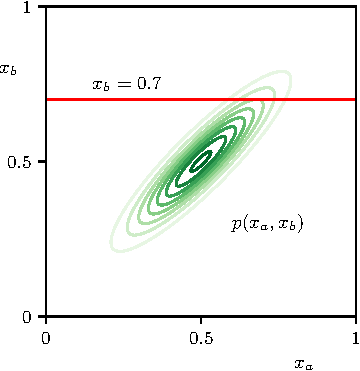
\includegraphics[scale=0.8]{./img/statistics/mv_gaussian.pdf}
		}{0.49}{
			\centering
			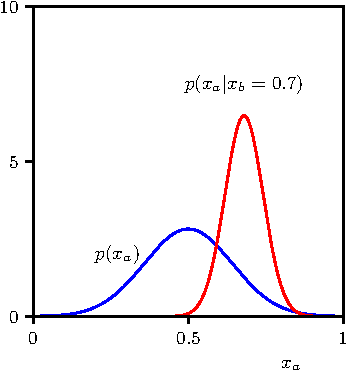
\includegraphics[scale=0.8]{./img/statistics/mv_gaussian_operations.pdf}
		}
		\caption{Links: Zweidimensionale Normalverteilung. Rechts: Randverteilung für $x_a$ in blau. Siehe \cite{Bishop2024}, Seite 82.}
	\end{figure}
\end{frame}


% Aufgabe: Normale Randverteilung
\begin{frame}{Aufgabe: Normale Randverteilung}{}
	\begin{mytask}
		Betrachten Sie erneut die Verbunddichte $p(X_1, X_2)$ wie sie in Aufgabe \ref{task:cond-norm} definiert wurde.
		
		Wie lautet die Dichte der Randverteilung $p(X_1)$?
	\end{mytask}
\end{frame}


% Satz von Bayes für Normalverteilungen
\begin{frame}{Satz von Bayes für Normalverteilungen}{}
	\begin{mytheo}[th:bayes-norm]
		Es seien $\bx$ und $\by$ Zufallsvektoren, sodass gilt
		\begin{equation*}
			\bx \sim \norm(\bmu, \bSigma)
		\quad\text{und}\quad
			\by \mid \bx \sim \norm(\bA \bx, \bLambda).
		\end{equation*}
		Dann gilt für die Verteilungen von $\by$ und $\bx \mid \by$
		\begin{align*}
			\by
				&\sim \norm\bigl( \bA \bmu, \bA \bSigma \bA^\top + \bLambda \bigr)
		\\[2mm]
			\bx \mid \by
				&\sim \norm\bigl( \bGamma [\bSigma^{-1} \bmu + \bA^\top \bLambda^{-1} \by], \bGamma \bigr).
		\end{align*}
		Hierbei ist $\bGamma \coloneqq \bigl( \bSigma^{-1} + \bA^\top \bLambda^{-1} \bA \bigr)^{-1}$.
	\end{mytheo}

	\begin{myproof}
		Einen Beweis dieser Aussage findet Sie in \cite{Bishop2006} auf den Seiten 90--93.
	\end{myproof}
\end{frame}


% SUBSECTION: Maximum-Likelihood Schätzer
\subsection{Maximum-Likelihood Schätzer}

% Maximum-Likelihood Methode
\begin{frame}{Maximum-Likelihood Methode}{}
	\begin{itemize}
		\item Im Folgenden sei ein Beobachtungsvektor $\bx \coloneqq \bigl( x_1, x_2, \ldots, x_N \bigr)^\top$
			bestehend aus $N$ \textit{unabhängig und identisch verteilten} (Englisch: \textit{independent and identically distributed} - i.\,i.\,d.)
				Datenpunkten gegeben.
		\item Wir möchten Aussagen über die Parameter $\btheta \coloneqq \bigl( \theta_1, \theta_2, \ldots, \theta_M \bigr)^\top$
			der zugrundeliegenden Verteilung machen.
		\item Dies erledigen wir durch eine Punktschätzung des Parametervektors $\btheta$. Den Schätzer für $\btheta$ bezeichnen wir mit $\bthetaest$.
		\item Eine der am häufigsten angewendete Methode ist die \keyword{Maximum-Likelihood Methode},
			die wir im Folgenden näher beleuchten werden.
	\end{itemize}
\end{frame}


% (Log-)Likelihood Funktion
\begin{frame}{(Log-)Likelihood Funktion}{}
	Der Maximum-Likelihood Schätzer $\bthetaestML$ für den Parametervektor $\btheta$ maximiert die Likelihood Funktion.
	
	\begin{mydef}[def:likelihood-function]
		Es sei $p(\bx; \btheta)$ die Dichte eines Zufallsvektors $\bx \in \R^N$, welche durch den Parametervektor $\btheta \in \Theta$ parametrisiert wird.
		Die \keyword{Likelihood Funktion} $L : \Theta \rightarrow \R$ ist dann definiert als
		\begin{equation*}
			L(\btheta) \coloneqq p(\bx; \btheta) = p(x_1, x_2, \ldots, x_N; \btheta).
		\end{equation*}
		Häufig ist es einfacher, die \keyword{Log-Likelihood Funktion} $l(\btheta) \coloneqq \ln p(\bx; \btheta)$ zu betrachten. \\
		Wir definieren $\bthetaestML \coloneqq \argmax_{\btheta} l(\btheta).$
	\end{mydef}

	\begin{boxGray}
		\textbf{Bemerkung:} Der Schätzer $\bthetaestML$ maximiert sowohl $L$ als auch $l$. \textbf{(Warum?)}
	\end{boxGray}
\end{frame}


% (Log-)Likelihood Funktion (Forts.)
\begin{frame}{(Log-)Likelihood Funktion (Forts.)}{}
	\begin{itemize}
		\item Im Allgemeinen kann es schwer sein, die Liklihood Funktion zu bestimmen
			\textit{(vor allem wenn die Beobachtungen voneinander abhängen)}.
		\item Die Annahme der \textbf{Unabhängigkeit der Beobachtungen} vereinfacht dies maßgeblich, denn
		\begin{align*}
			L(\btheta)
				&= p(x_1, x_2, \ldots, x_N; \btheta)
					= p(x_1; \btheta) \cdot p(x_2; \btheta) \cdot \ldots \cdot p(x_N; \btheta)
			\\[2mm]
				&= \prod_{n=1}^N p(x_n; \btheta).
		\end{align*}
		\item Für die Log-Likelihood Funktion ergibt sich durch Anwendung der Logarithmengesetze
		$$l(\btheta) = \ln \prod_{n=1}^N p(x_n; \btheta) = \sum_{n=1}^N \ln p(x_n; \btheta).$$
	\end{itemize}
\end{frame}


% Maximum-Likelihood Gleichung
\begin{frame}{Maximum-Likelihood Gleichung}{}
	\begin{itemize}
		\item Falls die Likelihood Funktion differenzierbar ist, so erfüllt der Maximum-Likelihood Schätzer $\bthetaestML$
			notwendig die \keyword{Likelihood Gleichung}
		\begin{equation*}
			\frac{\partial}{\partial \btheta} \ln p(\bx; \btheta)\,\bigg\vert_{\btheta = \bthetaestML} = \0.
		\end{equation*}
		\item Diese sagt aus, dass $\bthetaestML$ ein \textit{stationärer Punkt der (Log-)Likelihood Funktion} sein muss.
		\item Es handelt sich dabei um ein System von $M$, im Allgemeinen nicht-linearen, Gleichungen der Form
		\begin{equation*}
			\frac{\partial}{\partial \theta_j} \ln p(\bx; \btheta)\,\bigg\vert_{\btheta = \bthetaestML} = 0 \qquad j = 1, 2, \ldots, M.
		\end{equation*}
	\end{itemize}
	
	\begin{boxGray}
		\textbf{Achtung:} Es muss noch überprüft werden, ob $\bthetaestML$ tatsächlich ein Maximum darstellt.
	\end{boxGray}
\end{frame}


% Beispiel I: Binomialverteilung
\begin{frame}{Beispiel I: Binomialverteilung}{}
	\begin{mytheo}[th:mle-binomial]
		Es sei die binomialverteilte Zufallsvariable $X$ (Anzahl der Erfolge) und der Stichprobenumfang $N$ gegeben.
		Der Maximum-Likelihood Schätzer $\thetaestML$ für die unbekannte Erfolgswahrscheinlichkeit $\theta \in (0, 1)$ lautet
		$\thetaestML = \frac{k}{N}$, wobei $k$ die Anzahl der beobachteten Erfolge in der Stichprobe ist.
	\end{mytheo}
	
	\begin{myproof}
		Die Likelihood Funktion ist gegeben durch $L(\theta) = {N \choose k} \cdot \theta^k \cdot (1 - \theta)^{N - k}$.
		Wir wenden den Logarithmus an und erhalten die Log-Likelihood Funktion
		\begin{equation*}
			l(\theta) = \ln{N \choose k} + k \cdot \ln \theta + (N - k) \cdot \ln(1 - \theta).
		\end{equation*}
		Diese leiten wir nach $\theta$ ab und setzen sie Null. Auflösen nach $\theta$ ergibt schließlich
		\begin{equation*}
			\frac{\diff}{\diff \theta} l(\theta)
				= \frac{k}{\theta} - \frac{N - k}{1 - \theta}
				\overset{!}{=} 0
		\quad\Longleftrightarrow\quad
			\thetaestML
				= \frac{k}{N}.
		\end{equation*}
		Wir prüfen noch das Vorzeichen der zweiten Ableitung. Es ist
		$\frac{\diff^2}{\diff \theta^2} l(\theta) = -\frac{k}{\theta^2} - \frac{N - k}{(1 - \theta)^2} < 0\,\forall \theta \in (0, 1)$,
		sodass $\thetaestML$ tatsächlich ein Maximum ist. Es handelt sich sogar um ein global eindeutiges Maximum.
	\end{myproof}
\end{frame}


% Beispiel II: Normalverteilung
\begin{frame}{Beispiel II: Normalverteilung}{}
	\begin{mytheo}[th:mle-norm]
		Es seien $\bx = (x_1, x_2, \ldots, x_N)^\top$ \textit{unabhängig und identisch normalverteilte} Beobachtungen
		mit unbekanntem Erwartungswert $\mu \in \R$ und unbekannter Varianz $\sigma^2 > 0$.
		Der Parametervektor $\btheta$ ist in diesem Fall zweielementig und gegeben durch $\btheta \coloneqq \bigl( \mu, \sigma^2 \bigr)^\top$.
		
		Die Maximum-Likelihood Schätzer $\muML$ und $\sigmasquML$ für die unbekannten Parameter $\mu$ und $\sigma^2$
		werden in diesem Fall bestimmt mittels
		\begin{equation*}
			\muML
				= \frac{1}{N} \sum_{n=1}^n x_n
		\qquad\text{und}\qquad
			\sigmasquML
				= \frac{1}{N} \sum_{n=1}^N \bigl( x_n - \muML \bigr)^2.
		\end{equation*}
	\end{mytheo}
\end{frame}


% Beweis
\begin{frame}{}{}
	\begin{myproof}
		Die Dichte der Produktverteilung lautet aufgrund der Unabhängigkeit der Beobachtungen
		\begin{equation*}
			p\bigl( \bx; \mu, \sigma^2 \bigr)
				= \prod_{n=1}^N \frac{1}{\sqrt{2 \pi} \sigma} \cdot \exp\left( -\frac{(x_n - \mu)^2}{2 \sigma^2} \right)
				= \frac{1}{(2 \pi)^{\frac{N}{2}}} \cdot \frac{1}{\sigma^N} \cdot \exp\left( -\frac{\sum_{n=1}^N (x_i - \mu)^2}{2 \sigma^2} \right).
		\end{equation*}
		Aufgrund der auftretenden Exponentialverteilung bietet sich die Betrachtung der Log-Likelihood Funktion an. Wir erhalten
		\begin{equation*}
			l\bigl( \mu, \sigma^2 \bigr)
				= -\frac{N}{2} \cdot \ln(2 \pi) - N \ln(\sigma) - \frac{\sum_{n=1}^N (x_n - \mu)^2}{2 \sigma^2}.
		\end{equation*}
		Nun berechnen wir die partiellen Ableitungen von $l$ nach $\mu$ und $\sigma^2$. Es ist
		\begin{equation*}
			\frac{\partial}{\partial \mu} l\bigl( \mu, \sigma^2 \bigr)
				= \frac{1}{\sigma^2} \sum_{n=1}^N (x_n - \mu)
		\qquad\text{und}\qquad
			\frac{\partial}{\partial \sigma^2} l\bigl( \mu, \sigma^2 \bigr)
				= -\frac{N}{2 \sigma^2} + \frac{1}{2 \sigma^4} \sum_{n=1}^N (x_n - \mu).
		\end{equation*}
		Durch Nullsetzen und auflösen erhalten wir die im Satz angegebenen Maximum-Likelihood Schätzer $\muML$ und $\sigmasquML$.
		Es bleibt noch zu zeigen, dass es sich tatsächlich um ein Maximum handelt. Man rechnet nach,
		dass die Hesse-Matrix von $l\bigl( \mu, \sigma^2 \bigr)$ and der Stelle $\bigl( \muML, \sigmasquML \bigr)$ gegeben ist durch
		\begin{equation*}
			\nabla^2 l\bigl( \mu, \sigma^2 \bigr) =
			\begin{pmatrix}[1.3] -\frac{N}{\sigmasquML} & 0 \\ 0 & -\frac{N}{\bigl( \sigmasquML \bigr)^2} \end{pmatrix}.
		\end{equation*}
		Diese Matrix ist negativ definit, weshalb wir tatsächlich ein Maximum gefunden haben.
	\end{myproof}
\end{frame}


% Erwartungstreue Schätzer
\begin{frame}{Erwartungstreue Schätzer}{}
	Wir definieren den Begriff der Erwartungstreue:
	\begin{mydef}[def:unbiased-estimator]
		Wir nennen einen Schätzer $\bthetaest$ \keyword{erwartungstreu}, falls $\E\bigl[ \bthetaest \bigr] = \btheta$ gilt.
	\end{mydef}
	
	\begin{itemize}
		\item Der Schätzer $\muML$ ist erwartungstreu für den Erwartungswert $\mu$
		im Normalverteilungsmodell \\ \vspace*{2mm}
		\begin{myproof}
			Es gilt
			\begin{equation*}
				\E\bigl[ \muML \bigr]
					= \E\left[ \frac{1}{N} \sum_{n=1}^N x_n \right]
					= \frac{1}{N} \sum_{n=1}^N \E[x_n]
					= \frac{1}{N} \cdot N \cdot \mu
					= \mu.
			\end{equation*}
		\end{myproof}
		\item Demgegenüber ist $\sigmasquML$ \textbf{nicht} erwartungstreu.
			Man kann diesen Schätzer jedoch durch eine geeignete Transformation
			zu einem erwartungstreuen Schätzer machen. Dies führt auf die \keyword{empirische Varianz}
			$\frac{N}{N - 1} \sigmasquML = \frac{1}{N - 1} \sum_{n=1}^N \bigl( x_n - \muML \bigr)^2$.
	\end{itemize}
\end{frame}


% Aufgabe zur Maximum-Likelihood Schätzung
\begin{frame}{Aufgabe zur Maximum-Likelihood Schätzung}{}
	\begin{mytask}
		Gegeben seien die $N$ Beobachtungen $x_1, x_2, \ldots, x_N$, wobei $x_n \in \N, n = 1, 2, \ldots, N$.
		Sie legen den Daten eine Poisson-Verteilung zugrunde. Diese hat die Dichte
		\begin{equation*}
			p(x) \coloneqq e^{-\lambda} \cdot \frac{\lambda^x}{x!}.
		\end{equation*}
		
		\begin{enumerate}
			\item Bestimmen Sie den Maximum-Likelihood Schätzer $\lambdaML$ für die Poisson-Verteilung.
				Vergessen Sie dabei nicht zu überprüfen, ob es sich tatsächlich um ein Maximum handelt.
			\item Prüfen Sie den Schätzer auf Erwartungstreue.
		\end{enumerate}
	\end{mytask}
\end{frame}


% Erwartete quadratische Abweichung (MSE)
\begin{frame}{Erwartete quadratische Abweichung (MSE)}{}
	Ein weiteres Qualitätsmerkmal eines Schätzers $\thetaest$ ist seine erwartete quadratische
	Abweichung vom wahren Parameter $\theta$.
	
	\begin{mydef}[def:mse]
		Die \keyword{erwartete quadratische Abweichung} von $\thetaest$ zu $\theta$ ist
		\begin{equation*}
			\MSE\bigl[ \thetaest, \theta \bigr] = \E\left[ \bigl( \thetaest - \theta \bigr)^2 \right].
		\end{equation*}
	\end{mydef}
	
	Die $\MSE\bigl[ \thetaest, \theta \bigr]$ reduziert sich für erwartungstreue Schätzer $\thetaest$
	auf die Varianz $\V\bigl[ \thetaest \bigr]$. \\
	\vspace*{2mm}
	\begin{myproof}
		Man rechnet nach, dass
		$\MSE\bigl[ \thetaest, \theta \bigr] = \V\bigl[ \thetaest \bigr] + \bigl( \E\bigl[ \thetaest \bigr] - \theta \bigr)^2$ gilt
		(multipliziere hierzu aus und nutze die Linearität des Erwartungswerts).
		Der zweite Summand (Quadrat der Verzerrung/Bias) verschwindet aber für erwartungstreue Schätzer,
		da $\E\bigl[ \thetaest \bigr] = \theta$ gilt. Es folgt die Behauptung.
	\end{myproof}
\end{frame}


% SUBSECTION: Maximum-Aposteriori Schätzer
\subsection{Maximum-Aposteriori Schätzer}

% Maximum-Aposteriori Schätzer (MAP)
\begin{frame}{Maximum-Aposteriori Schätzer (MAP)}{}
	\begin{itemize}
		\item ML Schätzer laufen Gefahr, sich übermäßig stark an die Daten anzupassen (\keyword{Overfitting}).
		\item Wir erweitern daher das Konzept der ML Schätzung, indem wir zusätzlich eine \textit{Apriori-Verteilung}
			für die zu schätzenden Parameter mit einbeziehen.
		\item Wir nutzen den Satz von Bayes, um damit zusammen mit der Likelihood eine \textit{Aposteriori-Verteilung}
			über die Parameter zu erhalten.
		\item Ein Schätzer $\bthetaestMAP$ heißt \keyword{Maximum-Aposteriori Schätzer} für den Parameter $\btheta$,
			falls dieser die Aposteriori-Wahrscheinlichkeit maximiert.
	\end{itemize}
\end{frame}


% Binäre Variablen
\begin{frame}{Binäre Variablen}{}
	\begin{itemize}
		\item Wir betrachten eine binäre Zufallsvariable $X \in \{ 0, 1 \}$, z.\,B. das Werfen einer (unfairen) Münze,
			wobei $X = 1$ Kopf und $X = 0$ Zahl bedeutet.
		\item Die Zufallsvariable $X$ ist damit \keyword{Bernoulli-verteilt} mit der Dichte
		\begin{equation*} \label{eq:bernoulli}
			p_X(k) \coloneqq \mu^k \cdot (1 - \mu)^{1 - k}.
		\end{equation*}
		\item Es gilt
		\begin{align*}
			\E[X]
				&= \mu
		\\[2mm]
			\V[X]
				&= \mu \cdot (1 - \mu).
		\end{align*}
	\end{itemize}
	
	\begin{mytask}
		Beweisen Sie die Aussagen $\E[X] = \mu$ und $\V[X] = \mu \cdot (1 - \mu)$.
	\end{mytask}
\end{frame}


% Maximum Likelihood für die Bernoulli-Verteilung
\begin{frame}{Maximum Likelihood für die Bernoulli-Verteilung}{}
	\begin{itemize}
		\item Wir gehen nun von $N$ unabhängigen Bernoulli-verteilten Zufallsvariablen $X_1, X_2, \ldots, X_N$ aus.
		\item Dann ist die Likelihood Funktion für den Parameter $\mu$ gegeben durch
		\begin{equation*}
			L(\mu) = \prod_{n=1}^N p_{X_n}(k_n) = \prod_{n=1}^N \mu^{k_n} \cdot (1 - \mu)^{1 - k_n}.
		\end{equation*}
		\item Hieraus ergibt sich die Log-Likelihood Funktion
		\begin{equation*}
			l(\mu)
				= \sum_{n=1}^N \ln p_{X_n}(k_n)
				= \sum_{n=1}^N \bigl[ k_n \ln \mu + (1 - k_n) \cdot \ln(1 - \mu) \bigr]
				= \ln \mu \sum_{n=1}^N k_n + \ln(1 - \mu) \left( N - \sum_{n=1}^N k_n \right).
		\end{equation*}
	\end{itemize}
	
	\begin{boxGray}
		\textbf{Bemerkung:} Die Log-Likelihood Funktion hängt von den Beobachtungen nur über die Statistik \\
		$Y \coloneqq \sum_{n=1}^N X_n$ ab. Man nennt $Y$ daher eine \keyword{suffiziente Statistik}.
	\end{boxGray}
\end{frame}


% Maximum Likelihood für die Bernoulli-Verteilung (Forts.)
\begin{frame}{Maximum Likelihood für die Bernoulli-Verteilung}{}
	\begin{itemize}
		\item Leiten wir $l(\mu)$ nach $\mu$ ab und setzen Null, so erhalten wir den Maximum-Likelihood Schätzer als
			arithmetisches Mittel der Beobachtungen
		\begin{equation*}
			\muML = \frac{1}{N} \sum_{n=1}^N k_n.
		\end{equation*}
		\item Schreiben wir für die Anzahl der Erfolge (Kopf) $m \coloneqq \sum_{n=1}^N k_n$, so ist $\muML = \frac{m}{N}$.
		\item Werfen wir die Münze drei Mal und erhalten jedes Mal Kopf, so wäre $\muML = 1$ \textbf{(Overfitting)}.
		\item Die Zufallsvariable $Y \coloneqq X_1 + X_2 + \ldots + X_N$ ist aufgrund der Unabhängigkeit der $X_n$
			($1 \le n \le N$) \keyword{binomial-verteilt}, sodass gilt
		\begin{equation*}
			\Prob(Y = m) \coloneqq {N \choose m} \cdot \mu^m \cdot (1 - \mu)^{N - m}.
		\end{equation*}
	\end{itemize}
\end{frame}


% Beta-Verteilung
\begin{frame}{Beta-Verteilung}{}
	Um die Overfitting-Problematik zu adressieren, führen wir einen Beta-verteilten Prior ein.
	
	\begin{mydef}[def:beta-dist]
		Es sei $X$ eine \keyword{Beta-verteilte} Zufallsvariable, in Notation $X \sim \beta_{a, b}$, mit den Parametern
		$a, b > 0$. Die Dichte der Verteilung ist gegeben durch
		\begin{equation*}
			p_X(\xi)
				= \frac{\Gamma(a + b)}{\Gamma(a) \cdot \Gamma(b)}
					\cdot \xi^{a - 1} \cdot (1 - \xi)^{b - 1} \cdot \indicator_{(0, 1)}(\xi).
		\end{equation*}
	\end{mydef}
	
	\begin{boxGray}
		\textbf{Bemerkung:} $\Gamma(x)$ ist hierbei die \keyword{Gamma-Funktion}. Es gilt
		$\Gamma(x) \coloneqq \int_0^\infty u^{x-1} e^{-u}\,\diff u.$ Mithilfe partieller Integration kann man den Zusammenhang
		$\Gamma(x + 1) = x \cdot \Gamma(x)$ zeigen. Außerdem gilt $\Gamma(1) = 1$. Daraus folgt $\Gamma(n + 1) = n!$ für
		$n \in \N$. Somit ist die Gamma-Funktion die kontinuierliche Fortsetzung der Fakultäts-Funktion.
	\end{boxGray}
\end{frame}


% Visualisierung: Beta-Verteilung
\begin{frame}{Visualisierung: Beta-Verteilung}{}
	\begin{figure}[H]
		\divideTwo{0.49}{
			\centering
			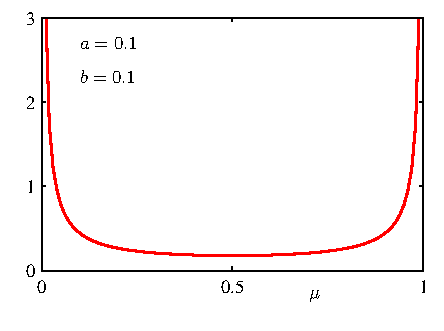
\includegraphics[scale=0.85]{./img/statistics/beta_1.pdf}
		}{0.49}{
			\centering
			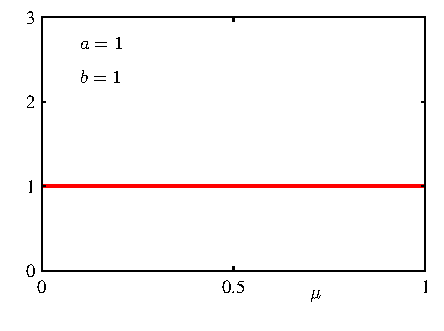
\includegraphics[scale=0.85]{./img/statistics/beta_2.pdf}
		}
		\caption{Beta-Verteilungen für einige Parameter $a, b$. Siehe \cite{Bishop2006}, Seite 72.}
	\end{figure}
\end{frame}


% Visualisierung: Beta-Verteilung (Forts.)
\begin{frame}{Visualisierung: Beta-Verteilung (Forts.)}{}
	\begin{figure}[H]
		\divideTwo{0.49}{
			\centering
			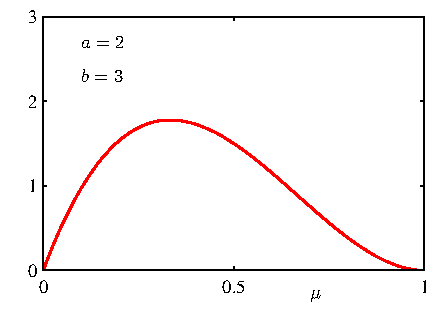
\includegraphics[scale=0.85]{./img/statistics/beta_3.pdf}
		}{0.49}{
			\centering
			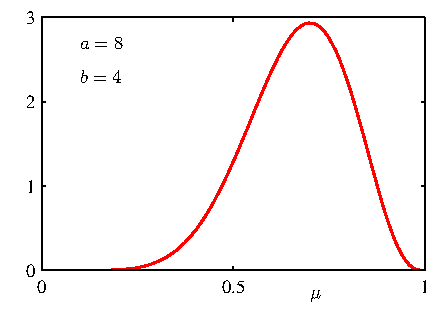
\includegraphics[scale=0.85]{./img/statistics/beta_4.pdf}
		}
		\caption{Beta-Verteilungen für einige Parameter $a, b$. Siehe \cite{Bishop2006}, Seite 72.}
	\end{figure}
\end{frame}


% Bestimmung des Posteriors
\begin{frame}{Bestimmung des Posteriors}{}
	\begin{itemize}
		\item Um den Posterior zu erhalten, multiplizieren wir den Beta-verteilten Prior mit der binomial-verteilten Likelihood.
		\item Ignorieren wir alle von $\mu$ unabhängigen Terme, so erhalten wir für den Posterior mit $l \coloneqq N - m$
			(Anzahl Misserfolge)
		\begin{equation} \label{eq:beta-post}
			p(\mu \mid m, l; a, b) \propto \mu^{m + a - 1} \cdot (1 - \mu)^{l + b - 1}.
		\end{equation}
		\item Da Prior und Likelihood \textit{dieselbe funktionale Form} haben, ist \textit{auch der Posterior wieder Beta-verteilt},
			wobei sich der Normierungsfaktor durch Vergleich mit der Dichte aus \ref{def:beta-dist} ergibt
		\begin{equation} \label{eq:beta-post-normalized}
			p(\mu \mid m, l; a, b)
				= \frac{\Gamma(m + a + l + b)}{\Gamma(m + a) \cdot \Gamma(l + b)}
					\cdot \mu^{m + a - 1} \cdot (1 - \mu)^{l + b - 1}
		\end{equation}
	\end{itemize}
	
	\begin{boxGray}
		Wir gehen also vom Prior mit der Dichte $\beta_{a, b}$ über zum Posterior mit der Dichte $\beta_{a + m, b + l}$.
	\end{boxGray}
\end{frame}


% Visualisierung: Bestimmung des Posteriors
\begin{frame}{Visualisierung: Bestimmung des Posteriors}{}
	\begin{figure}[H]
		\divideThree{0.32}{
			\centering
			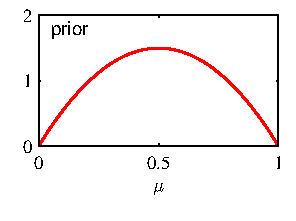
\includegraphics[scale=0.85]{./img/statistics/beta_prior.pdf}
		}{0.32}{
			\centering
			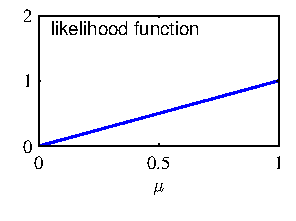
\includegraphics[scale=0.85]{./img/statistics/binomial_likelihood.pdf}
		}{0.32}{
			\centering
			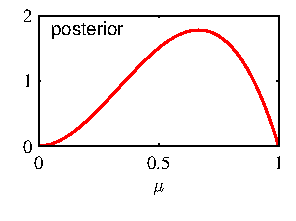
\includegraphics[scale=0.85]{./img/statistics/beta_posterior.pdf}
		}
		\caption{Ein Schritt der Bayes'schen Inferenz. Der Prior ist gegeben durch eine Beta-Verteilung mit $a = 2 = b$.
		Die Likelihood Funktion ist hingegen gegeben durch eine Binomial-Verteilung mit $N = m = 1$.
		Der Posterior ist damit wieder Beta-verteilt mit den Parametern $a = 3$ und $b = 2$. Siehe \cite{Bishop2006}, Seite 73.}
	\end{figure}
\end{frame}


% Konjugierte Verteilungen
\begin{frame}{Konjugierte Verteilungen}{}
	\begin{mydef}[def:conjugated-dist]
		Ein Prior heißt \keyword{konjugiert} zur Likelihood, wenn der daraus berechnete Posterior exakt dieselbe funktionale
		Form wie der Prior annimmt.
	\end{mydef}
	
	\begin{itemize}
		\item \textbf{Vorteil:} Der Posterior kann durch Aufdatierung der Parameter des Priors einfach bestimmt werden.
		\item Wichtige Paare:
		\begin{tabbing}
			\hspace*{0.5cm} \= \hspace*{4cm} \= \kill
			\> 	Binomial-Verteilung 	\> Beta-Verteilung \\
			\>	Poisson-Verteilung 	\> Gamma-Verteilung \\
			\>	Normalverteilung	\> Normalverteilung ($\mu$ zu schätzen, Varianz $\sigma^2$ bekannt)
		\end{tabbing}
	\end{itemize}
\end{frame}


% Aufgabe: Konjugierte Verteilungen
\begin{frame}{Aufgabe: Konjugierte Verteilungen}{}
	\begin{mytask}
		Weisen Sie nach, dass die Gamma-Verteilung den konjugierten Prior zur Likelihood der Poisson-Verteilung darstellt.
	\end{mytask}
\end{frame}


% Bestimmung des MAP-Schätzers
\begin{frame}{Bestimmung des MAP-Schätzers}{}
	\begin{itemize}
		\item Der MAP-Schätzer \textit{maximiert den Posterior} \eqref{eq:beta-post-normalized}.
		\item Der \keyword{Log-Posterior} lautet
		\begin{equation*}
			ln p( \mu \mid m, l; a, b) = (m + a - 1) \ln \mu + (l + b - 1) \ln (1 - \mu) + \const.
		\end{equation*}
		\item Ableiten nach $\mu$, Nullsetzen und Auflösen nach $\mu$ ergibt den MAP-Schätzer
		\begin{equation*}
			\muMAP = \frac{m + a - 1}{m + l + a + b - 2}.
		\end{equation*}
		\item Vergleich mit dem ML-Schätzer
		\begin{equation*}
			\muML = \frac{m}{m + l}.
		\end{equation*}
	\end{itemize}
\end{frame}


% SUBSECTION: Bayes'sche Inferenz
\subsection{Bayes'sche Inferenz}

% Bayes'sche Inferenz
\begin{frame}{Bayes'sche Inferenz}{}
	\begin{itemize}
		\item Wir haben $N$ Münzwürfe mit $m$ Erfolgen (Kopf) und $l$ Misserfolgen (Zahl) beobachtet.
		\item Unser Ziel ist es nun, den Ausgang des nächsten Wurfs vorherzusagen.
		\item Hierzu werten wir die \keyword{Prädiktivverteilung (Vorhersageverteilung)} aus
		\begin{align*}
			\Prob(X_{N+1} = 1 \mid m, l)
				&= \int_0^1 \Prob(X_{N+1} = 1 \mid \mu) \cdot p(\mu \mid m, l)\,\diff\mu
					= \int_0^1 \mu \cdot p(\mu \mid m, l)\,\diff\mu
		\\[2mm]
				&= \E[\mu \mid m, l].
		\end{align*}
		\item Der Erwarungswert des Posteriors können wir nun aus \eqref{eq:beta-post-normalized} ablesen, wir erhalten
		\begin{equation*}
			\Prob(X_{N+1} = 1 \mid m, l) = \frac{m + a}{m + a + l + b}.
		\end{equation*}
	\end{itemize}
\end{frame}